\chapter{How to Manage Stress and Mental Health?}

The source for this chapter is a School of Hard Knocks entrepreneurship interview curated for this course by LazyingArt LLC. The exchange is short, but it has a clear internal order. The interviewer asks how mental health, stress, and work-life balance are managed inside demanding positions. The answer does not begin with a technique. It begins with a principle: we need more than one focus in life. From there the speaker moves into his morning rhythm, the gym as mental space, hobbies as distance from the office, and finally the old image of sharpening the axe.

\section{The Question: Stress Inside Demanding Roles}

The opening question gives us the problem before it gives us any method. A demanding role creates pressure. If the role is allowed to occupy the whole field of attention, then the same focus that helps the work can also intensify the strain.

We can record the starting tension schematically:
\begin{equation}
\text{demanding role}
+
\text{continuous pressure}
\quad \Longrightarrow \quad
\text{stress risk}.
\end{equation}
This is not a psychological law. It is the situation the speaker is responding to. The interview asks how one manages that pressure while still living inside the position.

The answer will not be: work less, care less, or escape ambition. It will be subtler. We keep the work, but we do not let work become the only domain in which the person exists.

\section{More Than One Focus}

The first sentence of the answer is the hinge: one has to have more than one focus in life. Balance, in this account, is not primarily a calendar arrangement. It is a diversification of identity, effort, and attention.

A compact way to write the idea is:
\begin{equation}
\mathcal{F}
=
\{\text{work},\ \text{training},\ \text{hobbies}\}.
\end{equation}
The notation is our reconstruction, but the structure is transcript-backed. The speaker names work indirectly through the office and demanding positions; he then names training and hobbies as the other domains.

\subsection{Question \& Answer}

\paragraph{Question.}
If the business or position matters, why spend serious attention on anything outside it?

\paragraph{Answer.}
Because the person doing the work is part of the productive system. A life organized only around direct output has no explicit mechanism for renewing the person who produces that output. The speaker's answer treats training and hobbies not as decorative extras, but as ways of maintaining capacity.

We can express that mechanism cautiously as:
\begin{equation}
O_{\mathrm{sustained}}
\sim
E_{\mathrm{work}}\cdot C_{\mathrm{maintained}}.
\end{equation}
Here \(O_{\mathrm{sustained}}\) means durable output, \(E_{\mathrm{work}}\) means direct work effort, and \(C_{\mathrm{maintained}}\) means the maintained capacity of the person doing the work. The equation is not in the interview. It is a bookkeeping shorthand for the logic the interview states in practical language.

\section{The Morning Rhythm}

The answer then becomes concrete. The speaker says his rhythm is to get up at 4:30 in the morning and be in the gym by 5. The detail matters because the principle of multiple focuses is not left vague. It is built into the front of the day.

\begin{align}
t_{\mathrm{wake}} &= 4{:}30\ \mathrm{a.m.},\\
t_{\mathrm{gym}}  &= 5{:}00\ \mathrm{a.m.}.
\end{align}

He also gives the frequency. He generally works out seven days a week; some weeks are six; some days include two workouts:
\begin{align}
f_{\mathrm{workout}} &\approx 7\ \text{days/week},\\
f_{\mathrm{workout}} &\approx 6\ \text{days/week}\quad \text{on some weeks},\\
n_{\mathrm{workouts/day}} &= 2\quad \text{on some days}.
\end{align}

The point is not to universalize his schedule. The notes should not turn 4:30 a.m. into a moral rule. What matters is that the speaker has made physical practice regular enough to function as part of his operating system. The rhythm precedes the office, so the office does not get the first and only claim on his attention.

\section{Mind Space And Self-Directed Goals}

The next transition gives the reason for the rhythm. The gym gives him mind space. It is also a domain where he is pursuing goals that are his own.

That gives the gym a different role from mere exercise:
\begin{equation}
\text{training}
\quad \Longrightarrow \quad
\text{mind space}
+
\text{self-directed goals}.
\end{equation}
This is the local mechanism. The body is involved, but the claim is not only about the body. The gym is a place where the speaker can step outside the demands of the office and still remain in a disciplined, goal-seeking mode.

\begin{figure}
\centering
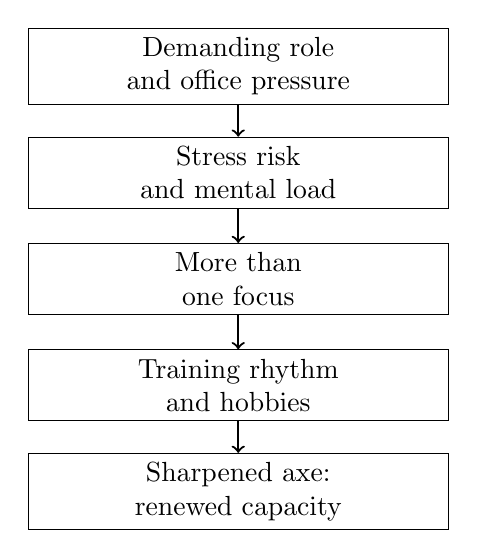
\begin{tikzpicture}[x=1cm,y=1cm]
\node[draw, rectangle, align=center, text width=5.1cm] (role) at (0,0)
{Demanding role\\and office pressure};
\node[draw, rectangle, align=center, text width=5.1cm] (risk) at (0,-1.35)
{Stress risk\\and mental load};
\node[draw, rectangle, align=center, text width=5.1cm] (focus) at (0,-2.70)
{More than\\one focus};
\node[draw, rectangle, align=center, text width=5.1cm] (practice) at (0,-4.05)
{Training rhythm\\and hobbies};
\node[draw, rectangle, align=center, text width=5.1cm] (capacity) at (0,-5.40)
{Sharpened axe:\\renewed capacity};

\draw[->, thick] (role) -- (risk);
\draw[->, thick] (risk) -- (focus);
\draw[->, thick] (focus) -- (practice);
\draw[->, thick] (practice) -- (capacity);
\end{tikzpicture}
\caption{A transcript-derived reconstruction of the answer's flow. No retained screenshot supplies a board diagram; this figure simply organizes the spoken sequence.}
\end{figure}

\section{Hobbies As Distance From The Office}

After the gym, the speaker widens the frame: he also has hobbies. He lists golf, sailing, hiking, and road biking. The list is not presented as a brand image or a lifestyle performance. It is presented as a set of ways to get away from the office.

\begin{table}
\centering
\begin{tabular}{p{0.30\linewidth} p{0.50\linewidth}}
\hline
Domain & Function in the answer \\
\hline
Gym rhythm & Mind space and a separate goal arena \\
Hobbies & Distance from the office environment \\
Office work & The demanding role that must be sustained \\
\hline
\end{tabular}
\caption{The speaker's examples divide life into domains with different functions.}
\end{table}

The golf detail is worth preserving: he says he does not play very well, but he likes to play. That keeps the point grounded. The hobby does not have to be another achievement arena. It can be valuable because it is a real place outside the office, with its own texture and attention.

\section{Sharpening The Axe}

The final move is the Abraham Lincoln anecdote. If Lincoln had four hours to chop down a tree, the saying goes, he would spend the first three sharpening the axe. The speaker uses the story to explain the role of the other activities. They sharpen the axe.

The ratio is easy to write:
\begin{align}
T_{\mathrm{total}}   &= 4\ \text{hours},\\
T_{\mathrm{sharpen}} &= 3\ \text{hours},\\
T_{\mathrm{chop}}    &= 1\ \text{hour}.
\end{align}
So the preparation share is:
\begin{equation}
\frac{T_{\mathrm{sharpen}}}{T_{\mathrm{total}}}
=
\frac{3}{4}.
\end{equation}

We should not read this as a literal allocation rule for every day. The speaker is not saying that three quarters of entrepreneurial life should be non-work. The point is structural: the tool must be maintained before the work can be done well. In this interview, the tool is the person.

\subsection{A Bookkeeping Example}

Let \(C_n\) denote usable personal capacity at the start of day \(n\). Let \(S_n\) denote the strain imposed by the day, and let \(R_n\) denote recovery from practices such as training, hobbies, and time away from the office. A minimal update rule is:
\begin{equation}
C_{n+1}=C_n-S_n+R_n.
\end{equation}

If there is strain without recovery, then over one week the schematic result is:
\begin{equation}
C_7
=
C_0-\sum_{n=0}^{6}S_n.
\end{equation}
If recovery is built into the week, the corresponding expression is:
\begin{equation}
C_7
=
C_0-\sum_{n=0}^{6}S_n
+
\sum_{n=0}^{6}R_n.
\end{equation}

This is the worked mathematical form of the axe metaphor. Stress draws down capacity. Recovery practices add something back. The speaker's gym routine and hobbies belong to \(R_n\). They are not the opposite of work; they are part of the maintenance of the worker.

\section{Summary}

The lecture begins with a question about stress, mental health, and work-life balance in demanding positions. The answer unfolds in order: have more than one focus, make the rhythm concrete, use training for mind space, keep hobbies that create distance from the office, and understand those practices as sharpening the axe.

The durable lesson is not that every entrepreneur should copy the same morning schedule. It is that sustained work requires maintained capacity. Direct effort matters, but the person doing the work must also be kept sharp.